\documentclass[a4paper,12pt]{article}

\usepackage{fontspec}
\setmainfont{Times New Roman}
\setmonofont[Scale=MatchLowercase]{Menlo}
\usepackage{unicode-math}
\setmathfont{STIX Two Math}
\usepackage[margin=2.5cm,columnsep=0.8cm]{geometry}
\usepackage{microtype}
\usepackage{setspace}
\usepackage{lineno}
\usepackage{fancyhdr}
\usepackage{ragged2e}
\usepackage{graphicx}
\usepackage{caption}
\DeclareCaptionFont{captionten}{\fontsize{10pt}{12pt}\selectfont}
\captionsetup{font={it,captionten},labelfont={bf,it},justification=centering,singlelinecheck=false}
\usepackage{booktabs}
\usepackage{tabularx}
\usepackage{longtable}
\usepackage{array}
\usepackage{xurl}
\usepackage[authoryear,round]{natbib}

\graphicspath{{../}}
\urlstyle{same}
\def\UrlFont{\rmfamily}
\renewcommand{\figurename}{Fig.}
\renewcommand{\topfraction}{0.95}
\renewcommand{\bottomfraction}{0.85}
\renewcommand{\textfraction}{0.05}
\renewcommand{\floatpagefraction}{0.85}
\makeatletter
\setlength{\@fptop}{0pt}
\setlength{\@fpsep}{10pt plus 2pt minus 2pt}
\setlength{\@fpbot}{0pt plus 1fil}
\makeatother

\setstretch{1.5}
\setlength{\parindent}{0pt}
\setlength{\parskip}{6pt}
\setlength{\emergencystretch}{1em}

\pagestyle{fancy}
\fancyhf{}
\fancyfoot[C]{\thepage}
\renewcommand{\headrulewidth}{0pt}
\renewcommand{\footrulewidth}{0pt}

\renewenvironment{abstract}
  {\section*{Abstract}\noindent\ignorespaces}
  {\par\medskip}

\begin{document}

\title{\fontsize{16pt}{19.2pt}\selectfont\textbf{Beyond thermal accumulation: improving cross-regional grapevine phenology prediction with terrain-aware forcing and residual learning}}

\author{}
\date{}

\maketitle
\vspace{-2.0\baselineskip}

\begingroup
\setlength{\parindent}{0pt}
\setlength{\parskip}{0.35\baselineskip}
Linjia Yao\textsuperscript{a}, Qiang Yu\textsuperscript{b}, Gang Zhao\textsuperscript{b,*}

\textsuperscript{a} College of Natural Resources and Environment, Northwest A\&F University, Yangling 712100, China

\textsuperscript{b} State Key Laboratory of Soil and Water Conservation and Desertification Control, College of Soil and Water Conservation Science and Engineering, Northwest A\&F University, Yangling, Shaanxi 712100, China

\textsuperscript{*} Corresponding author: Gang Zhao, E-mail: gang.zhao@nwafu.edu.cn
\par
\endgroup

\linenumbers
\justifying
\setlength{\parindent}{0pt}

\begin{abstract}
Accurate prediction of grapevine phenology across regions requires models that account for temperature responses, local terrain and systematic prediction errors. A European dataset contains 75,233 observations of budburst (BBCH07), flowering (BBCH65), veraison (BBCH81) and maturity/harvest (BBCH89) from 3,198 monitoring sites in 11 countries during 1951--2026. Observations were selected using directly recorded BBCH codes, exact-duplicate removal and checks of seasonal timing and intervals between developmental stages. The modelling framework combines linear or beta forcing, alternative chilling responses with sequential or parallel coupling, and optional machine-learning correction of process-model residuals. Each structure receives raw or elevation-corrected temperature, giving 40 configurations per stage. Calibration and testing are separated by site within temperature zones derived from climatic clustering, and residual models are trained on out-of-fold process predictions. Additional spatial and warm-climate tests assess transferability. Paired comparisons across elevation differences, slope, aspect and local terrain variability assess where temperature correction improves phenological predictions and whether residual learning modifies these gains. The observation dataset has been prepared; model evaluation remains to be completed.
\end{abstract}

\noindent\textit{Keywords:} Grapevine; BBCH; phenology; data quality; process-based model; elevation correction; residual learning; environmental transfer
\par\medskip

\section{Introduction}

Grapevine phenology regulates the seasonal timing of growth and reproduction, shaping exposure to frost, heat and water limitation as well as the scheduling of vineyard operations \citep{jonesClimateInfluencesGrapevine2000,tomasiGrapevinePhenologyClimate2011}. Earlier budburst can alter spring frost exposure, while shifts in flowering, veraison and ripening change the climatic conditions experienced during fruit development. Warming therefore affects both the suitability of wine-growing regions and the choice of cultivars and management practices \citep{vanleeuwenClimateChangeImpacts2024}. Reliable phenological predictions are essential for assessing seasonal development across contrasting growing environments.

Process-based phenology models predict developmental stages by accumulating temperature-dependent rates until specified requirements are reached \citep{chuineProcessBasedModelsPhenology2017}. Forcing-only models represent heat accumulation from a prescribed or calibrated date without explicitly simulating dormancy. Examples include growing degree days (GDD) and the Grapevine Flowering Veraison (GFV) model \citep{parkerGeneralPhenologicalModel2011a}. Chilling--forcing models additionally represent the cold exposure associated with dormancy release. In sequential models, forcing begins only after a chilling requirement is fulfilled; in parallel models, chilling and forcing can accumulate over overlapping periods, with forcing effectiveness potentially depending on chilling status \citep{chuineUnifiedModelBudburst2000}.

Within these families, temperature-response functions provide another dimension of model complexity. Forcing can increase linearly above a base temperature, approach a plateau through a sigmoid function, or decline above an optimum through a beta function. Chilling responses range from threshold-based accumulation to triangular and smooth nonlinear functions; triangular formulations developed for trees require evaluation for grapevine \citep{chuineUnifiedModelBudburst2000}. \citet{filaComparisonDifferentModelling2014} compared linear and beta forcing-only models with beta-based chilling--forcing models, allowing temperature-response parameters to be shared or vary among stages. Together with evidence that base-temperature selection can matter more than explicit dormancy representation \citep{garciadecortazar-atauriPerformanceSeveralModels2009}, these findings favour independent evaluation of model components rather than assuming that greater complexity improves prediction.

Hybrid approaches offer a complementary route to improved prediction by combining process-based models with machine learning \citep{reichsteinDeepLearningProcess2019}. Residual learning retains the process-model prediction and estimates its systematic error from additional environmental covariates. This can represent statistical associations omitted from a temperature-driven formulation, but does not establish the underlying physiological mechanisms. Its usefulness depends on whether the correction transfers beyond the conditions represented during calibration. Spatially dependent observations can make random record-level validation overoptimistic, reinforcing the need for evaluation at independent sites and under contrasting environmental conditions \citep{robertsCrossvalidationStrategiesData2017}.

Temperature representativeness adds uncertainty in complex terrain, where regional weather stations and gridded climate fields cannot fully resolve vineyard-scale conditions. Elevation, slope exposure and cold-air drainage produce local temperature contrasts that influence phenological timing \citep{neethlingSpatialComplexityTemporal2019,deresseguierTemperatureVariabilityLocal2020}. Elevation-based adjustments offer a simple means of accounting for part of this spatial mismatch, although they cannot fully describe inversions, aspect effects or canopy microclimates. Consequently, the value of increasing process-model complexity or adding residual learning may depend on how well the temperature input represents the growing environment.

This study examines three complementary approaches to improving grapevine phenology prediction across contrasting European environments. The objectives are to (i) evaluate how process-based model structure, including forcing and chilling functions and their sequential or parallel interaction, affects predictive accuracy and environmental transferability; (ii) assess whether residual machine learning improves process-based predictions and whether its benefits depend on model structure; and (iii) quantify whether DEM-based elevation correction of temperature improves predictions, both alone and in combination with residual learning.

\section{Materials and methods}

\subsection{Overall workflow}

The overall workflow comprises five linked components (Fig.~\ref{fig:study_framework}). Quality-controlled observations of BBCH07, BBCH65, BBCH81 and BBCH89 are matched to daily ERA5-Land temperature and terrain information (Fig.~\ref{fig:study_framework}a). Raw and DEM-corrected temperatures provide paired forcing inputs (Fig.~\ref{fig:study_framework}b). Each input is combined with linear or beta forcing, no chilling or alternative chilling responses, and optional residual machine learning. Sequential and parallel interactions are compared for models with chilling, yielding 40 candidate configurations per stage (Fig.~\ref{fig:study_framework}c).

All adjustable process parameters and residual learners are fitted within the calibration set; residual training uses out-of-fold process predictions. Locked configurations are evaluated at held-out sites stratified by clustered temperature zones, with additional spatial and warm-climate transfer tests (Fig.~\ref{fig:study_framework}d). Paired differences in test error quantify the contribution of elevation correction across terrain conditions and its interaction with residual learning (Fig.~\ref{fig:study_framework}e). Observation preparation is complete; model evaluation remains prospective.

\begin{figure}[!p]
\centering
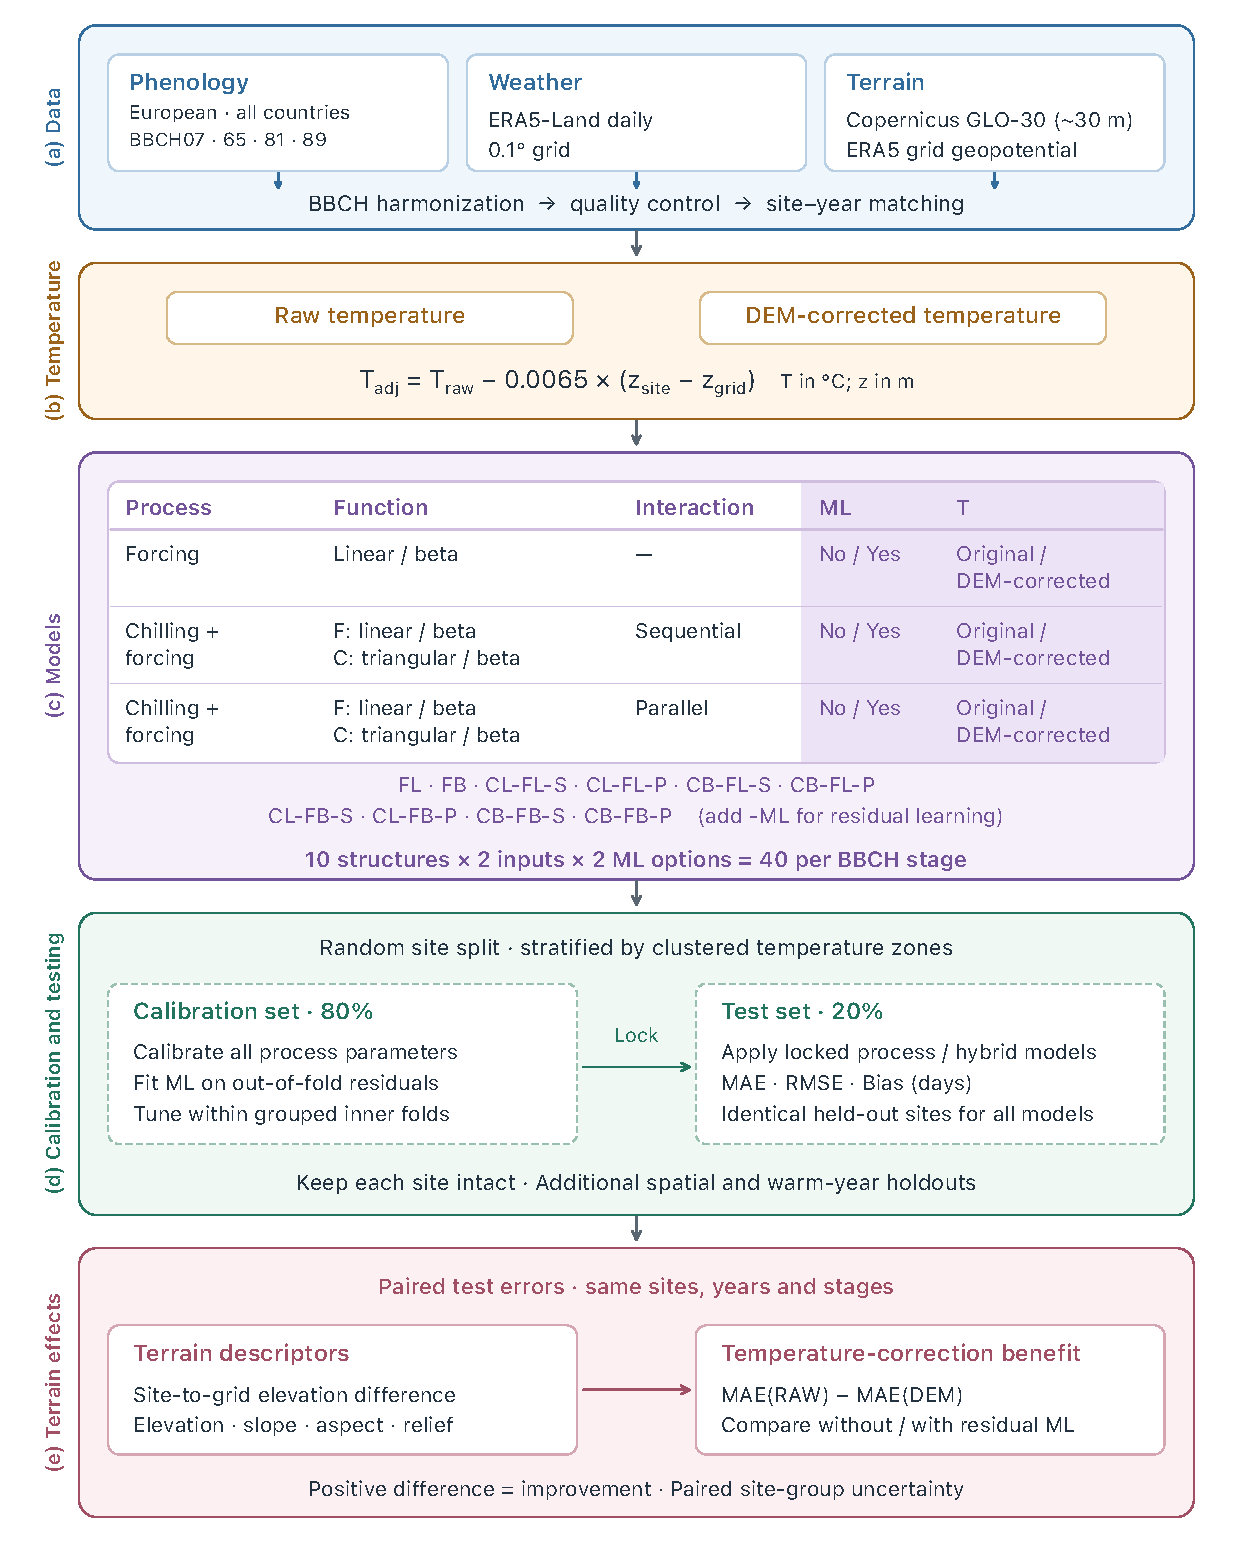
\includegraphics[width=0.92\textwidth,height=0.82\textheight,keepaspectratio]{fig/workflow/workflow.pdf}
\caption{Overall workflow for evaluating grapevine phenology models, residual learning and terrain-related prediction errors. (a) Phenology, weather and terrain data preparation; (b) paired raw and DEM-corrected temperatures; (c) factorial combinations of forcing, chilling, process interaction and residual learning; (d) calibration and independent testing within clustered temperature zones; and (e) paired prediction-error contrasts across terrain conditions. Model evaluation is prospective. DEM, digital elevation model; ML, machine learning; MAE, mean absolute error; RMSE, root mean squared error; DOY, day of year.}
\label{fig:study_framework}
\end{figure}

\clearpage
\subsection{Study area}

Grapevine observations were compiled for 3,198 monitoring sites across 11 European countries (Fig.~\ref{fig:study_area}). The sites extend from 38.10 to 59.15$^{\circ}$N and from 4.29$^{\circ}$W to 22.43$^{\circ}$E. Most are in France (1,639) and Germany (1,384), with additional sites in Switzerland, Slovakia, Croatia, Spain, Bosnia and Herzegovina, Czechia, Montenegro, Luxembourg and Sweden.

The main observation regions encompass contrasting temperate climates. Western France is strongly influenced by the Atlantic, with relatively mild temperatures and rainfall throughout the year, whereas Mediterranean France has hotter, drier summers. Northeastern France and Germany experience stronger continental influences and larger seasonal temperature contrasts. These regional patterns are modified by elevation, distance from the coast and mountain barriers \citep{meteofranceClimateFrance2023,dwdNationalClimateReport}.

The regional landscape includes lowlands, river valleys, hills and mountain foothills. Within wine-growing areas, slope and aspect influence solar exposure, while cold-air drainage can lower night-time temperatures in valleys and depressions. These local differences affect frost exposure and the timing of grapevine development, even within a single wine region. Soil conditions and water availability further differentiate growing environments and influence vineyard management \citep{deresseguierTemperatureVariabilityLocal2020}.

Grape-growing conditions range from cool regions, where sufficient heat for ripening and frost avoidance are important constraints, to warmer regions exposed to summer drought and excessive heat. Cultivar and rootstock selection, vine training and harvest timing are adapted to local climatic and soil conditions \citep{deresseguierTemperatureVariabilityLocal2020}. Warming can improve ripening opportunities in cooler areas but advance maturity and intensify water stress in already warm regions \citep{vanleeuwenClimateChangeImpacts2024}. These contrasts are relevant to both regional phenology prediction and the assessment of model performance under changing climates.

\begin{figure}[!p]
\centering
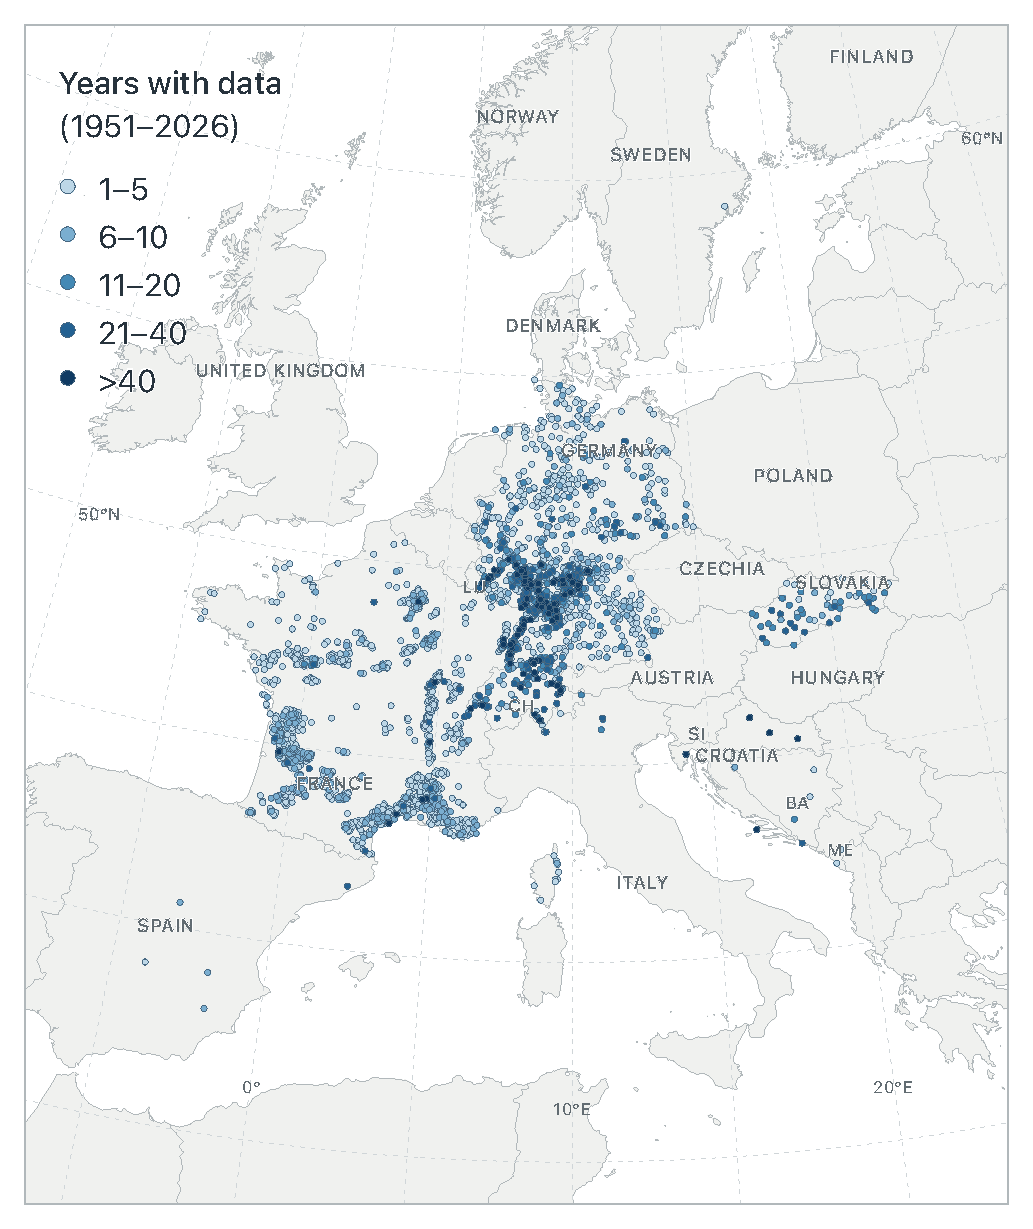
\includegraphics[width=\textwidth,height=0.78\textheight,keepaspectratio]{fig/study_area/study_area.pdf}
\caption{Study area and length of the grapevine phenology records. The map shows 3,198 sites reported by monitoring networks in 11 European countries. Colours indicate the number of years with at least one observation of BBCH07, BBCH65, BBCH81 or BBCH89 during 1951--2026, pooled across varieties. Sites reported by different networks may share a location.}
\label{fig:study_area}
\end{figure}

\clearpage
\subsection{Data}

\subsubsection{Phenology observations}

Grapevine observations were compiled from the TEMPO data portal \citep{mauryTempoDataPortal2023}, the Deutscher Wetterdienst (DWD) phenological database \citep{kasparPhenologicalNetworkDWD2014} and the Pan European Phenological database (PEP725) \citep{templPanEuropeanPhenological2018}. Data were provided by the members of the PEP725 project; the PEP725 dataset was accessed on 1 July 2026. A single version of each source dataset was used to avoid duplicating records from overlapping extracts or historical releases. Information on data providers and licences was retained where available.

Each observation includes the monitoring site, reported variety, country, latitude, longitude, date and BBCH stage. Site codes were retained separately for each network. Sites reported by different networks may share coordinates; their records were retained separately during data compilation. Reported site counts therefore do not necessarily represent independent vineyards. Records referring to the same physical location will be grouped together before model validation.

Country information and geographic coordinates were retained from the source datasets, with coordinates expressed in WGS84 decimal degrees. Only observations with directly recorded BBCH codes were retained; stages requiring an inferred conversion were excluded. Stage definitions followed the grapevine BBCH scale \citep{lorenzGrowthStagesGrapevine1995}. Dates and stage codes were standardized without interpolation or reassignment. Missing variety information was left unspecified, and DWD maturity classes were retained without interpreting them as named cultivars.

\paragraph{Data compilation and duplicate removal.}
The source datasets contained 823,028 records before filtering. Grapevine observations with directly recorded BBCH codes from 1 January 1951 onward were selected. Exact duplicates were removed when site, variety, country, coordinates, date and stage all agreed. Observations with different dates or varieties were retained separately, including repeated observations of the same stage within a year. Dates were not replaced by an earliest observation, median or other summary. These steps yielded 271,032 observations before seasonal and chronological screening.

All records remained linked to their original data source and quality-control outcome. Excluded observations were retained separately with the reason for exclusion and, where relevant, the dates used to assess stage order and phase duration. Counts were checked at each processing step to ensure that retained, duplicate and excluded records accounted for the original datasets.

\begin{table}[!htbp]
\centering
\caption{Number of records retained during data preparation. The initial total includes repeated records from the source datasets; subsequent counts refer to unique observations.}
\label{tab:data_flow}
\small
\setlength{\tabcolsep}{5pt}
\begin{tabularx}{\textwidth}{>{\raggedright\arraybackslash}X>{\raggedleft\arraybackslash}p{0.22\textwidth}>{\raggedright\arraybackslash}p{0.34\textwidth}}
\toprule
Processing step & Records & Description \\
\midrule
Source datasets & 823,028 & Includes repeated records and observations later excluded \\
Date and BBCH filtering, followed by duplicate removal & 271,032 & Grapevine observations with directly recorded BBCH codes from 1951 onward \\
Excluded by seasonal and chronological screening & 11,034 (4.1\%) & Observations outside the date or interval criteria \\
Retained observations, all stages & 259,998 & 4,244 reported sites in 13 countries \\
Selected modelling stages & 75,233 & BBCH07, BBCH65, BBCH81 and BBCH89 \\
\bottomrule
\end{tabularx}
\end{table}

\paragraph{Phenological quality control.}
Seasonal timing and the order and duration of developmental phases were checked after duplicate removal. The screening thresholds were defined for this European dataset; they are not universal physiological limits and were not derived from model residuals. Observed dates and stage codes were not corrected, and the thresholds are not imposed on model predictions.

Observations were first checked against stage-specific calendar windows, with both boundary dates included (Table~\ref{tab:seasonal_windows}). Dates were compared by month and day so that leap years were treated consistently. No seasonal window was imposed on BBCH00 or BBCH90--99, because dormancy and late-season development can extend across calendar years, or on stages outside the groups listed in the table.

\begin{table}[!htbp]
\centering
\caption{Seasonal windows used to screen phenological observations. Boundary dates are included.}
\label{tab:seasonal_windows}
\small
\setlength{\tabcolsep}{5pt}
\begin{tabularx}{\textwidth}{>{\centering\arraybackslash}p{0.16\textwidth}>{\raggedright\arraybackslash}X>{\raggedright\arraybackslash}p{0.34\textwidth}}
\toprule
BBCH family & Stage group & Eligible dates \\
\midrule
01--09 & Bud development & 1 February--15 June \\
10--19 & Leaf development & 1 March--31 July \\
50--59 & Inflorescence development & 1 April--15 July \\
60--69 & Flowering & 1 May--31 July \\
70--79 & Fruit development & 15 May--15 September \\
80--85 & Veraison/early ripening & 1 July--15 October \\
86--89 & Late ripening/maturity & 15 July--15 November \\
\bottomrule
\end{tabularx}
\end{table}

Stage order and phase duration were assessed within each site, reported variety and calendar year. Observations without a variety name were grouped separately from named cultivars. These groups, and those defined by DWD maturity classes, may include several plants or cultivars, so inconsistent dates cannot necessarily be attributed to an error in an individual plant.

Two developmental sequences were assessed separately: bud and leaf development (BBCH01, 03, 05, 07, 09 and 10--19) and reproductive development (BBCH01, 03, 05, 07, 09, 53, 55, 57, 60--69, 71, 73, 75, 77, 79, 81, 83, 85, 87 and 89). All observed stage pairs within each sequence were compared. Separate sequences allowed leaf and reproductive development to overlap without imposing an order based solely on their numerical BBCH codes. BBCH00 and BBCH90--99 were excluded from these comparisons.

A later stage could occur on the same date as an earlier stage, but not before it. Additional minimum and maximum intervals were applied between budburst and flowering, flowering and veraison, and veraison and maturity (Table~\ref{tab:phase_intervals}). BBCH07 and BBCH09 were treated as distinct budburst observations. The interval rules applied only to the listed stages; missing stages were neither inferred nor grounds for exclusion.

\begin{table}[!htbp]
\centering
\caption{Acceptable intervals between major developmental stages for data screening. Both limits are included.}
\label{tab:phase_intervals}
\small
\begin{tabular}{ccc}
\toprule
Earlier stage & Later stage & Inclusive interval (d) \\
\midrule
BBCH07 or BBCH09 & BBCH65 & 20--100 \\
BBCH65 & BBCH81 & 30--120 \\
BBCH81 & BBCH89 & 10--90 \\
\bottomrule
\end{tabular}
\end{table}

Interval checks were applied to observations that passed the seasonal screen. For each pair of observed stages, every date required at least one date at the other stage that satisfied the interval criterion. A date that failed this check was excluded even if another observation of the same stage was compatible. When no compatible pair existed, observations of both stages were excluded because the erroneous date could not be identified. All exclusions were determined from the same set of observations and applied simultaneously in each iteration. Checks were repeated until no further exclusions occurred. Stages with no remaining observations imposed no additional constraint, and unrelated stages were retained. Screening excluded 11,034 observations (4.1\%), leaving 259,998 observations. Excluded records remain available for sensitivity analysis because unusual weather, reporting intervals and management practices may also produce atypical dates.

\paragraph{Modelling stages.}
The modelling dataset contains 75,233 observations: 25,303 of budburst (BBCH07), 26,657 of flowering (BBCH65), 18,734 of veraison (BBCH81) and 4,539 of maturity/harvest (BBCH89). Records of other stages remain in the consolidated dataset but are not included in the model comparisons.

Observations cover 1951--2026, with 1--72 years of data per site. Record length is defined as the number of years with at least one observation, irrespective of gaps between years. Sites and years with observations of any one of the four stages were retained; complete developmental sequences and a minimum record length were not required. Interpretation of BBCH89 depends on the source definition, because harvest timing may reflect management decisions as well as physiological maturity.

\subsubsection{Temperature data}

Historical weather inputs are based on daily ERA5-Land data at 0.1$^{\circ}$ resolution. Variables include daily mean, minimum and maximum 2-m air temperature, 2-m dew-point temperature, total precipitation, surface pressure, downward solar radiation and the two horizontal components of 10-m wind. The extraction period generally extends from 1 September of the preceding year to 31 December of the observation year, covering both chilling and subsequent development.

Phenology observations will be matched to weather and terrain data before modelling. Weather series must cover the full period required by each model, including the preceding chilling season, and pass checks for missing values, duplicate dates, units and physical consistency. All model comparisons will use the same observations and calibration--test assignments. Records from the same site or physical location, and sites sharing an ERA5-Land grid cell, will remain together during validation.

\subsubsection{Digital elevation model}

Site elevation and terrain characteristics are based on the Copernicus GLO-30 digital elevation model. ERA5-Land grid elevation is derived from its invariant geopotential using a gravitational acceleration of 9.80665~m~s$^{-2}$. This elevation represents the terrain used by the weather model and is distinct from the mean GLO-30 elevation within a grid cell. Elevations reported by the observation networks are retained for comparison, while GLO-30 provides a common terrain dataset across countries.

\subsubsection{DEM-based temperature correction}

Each model is evaluated with raw and elevation-corrected temperatures. The correction is applied to daily mean, minimum and maximum temperature:

\begin{equation}
T_{\mathrm{DEM},d}=T_{\mathrm{RAW},d}-0.0065\left(z_{\mathrm{site}}-z_{\mathrm{grid}}\right),
\label{eq:temperature_adjustment}
\end{equation}

where temperature is expressed in $^{\circ}$C, $z_{\mathrm{site}}$ is the GLO-30 site elevation and $z_{\mathrm{grid}}$ is the ERA5-Land grid elevation, both in metres. A lapse rate of 6.5~$^{\circ}$C~km$^{-1}$ gives a $-0.65~^{\circ}$C adjustment for a site 100~m above the grid elevation. Other meteorological variables are unchanged. Any alternative lapse rate estimated from observations will be fitted within the calibration folds. Forcing and chilling requirements are recalibrated separately for raw and corrected temperatures using the same observations, while temperature-response parameters remain identical. The comparison therefore assesses prediction after threshold recalibration, rather than the temperature correction alone. Improved phenology predictions would not, by themselves, demonstrate greater accuracy of the corrected temperatures.

\subsection{Models}

\subsubsection{Process-based phenology models}

Six function combinations pair two forcing functions with three chilling options (Table~\ref{tab:model_catalogue}). The two forcing-only combinations and sequential and parallel variants of the four chilling--forcing combinations give ten process-model structures. Linear forcing (FL) accumulates thermal time above a fixed base temperature. Beta forcing (FB) represents a nonlinear response that peaks at an optimum temperature and declines to zero at the upper temperature limit. Beta forcing and beta chilling (CB) follow the response families examined by \citet{filaComparisonDifferentModelling2014}. Piecewise-linear chilling (CL) uses the triangular response described by \citet{deWergifosseHETEROFOR2020}, following H\"anninen (1990). This chilling function was developed for forest trees; its application to grapevine is an adaptation. Temperature-response parameters are fixed from literature and shared across stages, sites and models wherever the same component occurs; only accumulation requirements are calibrated.

\paragraph{Daily temperature responses.}
All process models use daily mean air temperature $T_t$ in $^{\circ}$C. For target stage $s\in\mathcal{S}=\{07,65,81,89\}$, linear forcing is

\begin{equation}
R^{\mathrm{FL}}_{f,s}(T_t)=\max(T_t-T_b,0),
\label{eq:linear_forcing}
\end{equation}

where $T_b=0$~$^{\circ}$C for all stages, following the base temperature of the GFV model \citep{parkerGeneralPhenologicalModel2011a}. GFV originally targets flowering and veraison; use of this base for the complete four-stage sequence is an extension, not an exact reproduction of GFV. Summation over daily time steps gives thermal time in $^{\circ}$C\,d. The normalized beta response is

\begin{equation}
B(T;a,b,c)=
\begin{cases}
\displaystyle\frac{c-T}{c-b}
\left(\frac{T-a}{b-a}\right)^{\!\frac{b-a}{c-b}}, & a<T<c,\\[6pt]
0, & T\leq a\ \text{or}\ T\geq c,
\end{cases}
\label{eq:beta_response}
\end{equation}

where $a<b<c$ are the minimum, optimum and maximum temperatures, respectively, and $B(b;a,b,c)=1$ \citep{filaComparisonDifferentModelling2014}. Beta forcing uses $R^{\mathrm{FB}}_{f,s}(T_t)=B(T_t;0,25.4,35)$ for every stage. The optimum of 25.4~$^{\circ}$C is the shared forcing optimum of Fila et al.'s Fbeta5* model (Table~8), calibrated using field and growth-room observations; the lower and upper limits of 0 and 35~$^{\circ}$C follow their adopted beta formulation. Beta chilling uses $R^{\mathrm{CB}}_c(T_t)=B(T_t;T_{c,\min},T_{c,\mathrm{opt}},T_{c,\max})$. Its fixed cardinal temperatures are $-1.7$, 1.7 and 13.2~$^{\circ}$C, respectively, from the CF10* parameterization informed by field and growth-room observations in their Table~7. The alternative CL response is

\begin{equation}
R^{\mathrm{CL}}_c(T)=
\begin{cases}
0, & T\leq T_{c,\min}\ \text{or}\ T\geq T_{c,\max},\\[3pt]
\dfrac{T-T_{c,\min}}{T_{c,\mathrm{opt}}-T_{c,\min}}, & T_{c,\min}<T\leq T_{c,\mathrm{opt}},\\[6pt]
\dfrac{T_{c,\max}-T}{T_{c,\max}-T_{c,\mathrm{opt}}}, & T_{c,\mathrm{opt}}<T<T_{c,\max}.
\end{cases}
\label{eq:triangular_chilling}
\end{equation}

CL uses the same three chilling temperatures as CB, so the contrast changes curve shape without changing its temperature limits or optimum (Fig.~\ref{fig:temperature_responses}). These cardinals originate from grapevine beta chilling, not from the forest-tree parameterization of the triangular function. Both chilling responses are bounded between zero and one. Their cumulative sums, and those of beta forcing, are expressed as accumulated daily response units; they are not interchangeable with the degree-day sums of linear forcing.

\paragraph{Accumulation and stage progression.}
Each site--year is simulated independently through 31 December of the observation year. Forcing-only models start on 1 January ($t_0=1$), a common calendar convention discussed by \citet{filaComparisonDifferentModelling2014}. This date is fixed across sites, years and forcing functions, and differs from the day-60 origin of the original GFV model. The first day contributes to accumulation. Calendar start dates are not calibrated in the structure comparison.

For a stage starting on date $\tau_s$, cumulative effective forcing and its predicted occurrence date are

\begin{equation}
F_s(t)=\sum_{u=\tau_s}^{t}w_{s,u}R_{f,s}(T_u),\qquad
\widehat{D}_s=\min\{t\geq\tau_s:F_s(t)\geq H_s\},
\label{eq:stage_accumulation}
\end{equation}

where $H_s>0$ is the stage-specific forcing requirement and $w_{s,u}=1$ except during budburst forcing in parallel models. After each predicted stage, the forcing sum is reset to zero and accumulation for the next stage begins on the following day: $\tau_{65}=\widehat{D}_{07}+1$, $\tau_{81}=\widehat{D}_{65}+1$ and $\tau_{89}=\widehat{D}_{81}+1$. Threshold overshoot is discarded, and no day's forcing contributes to two stages. The four requirements therefore describe successive developmental intervals, not cumulative thresholds from a common starting date. Observed preceding-stage dates never initialize predictions, including during calibration or when intermediate observations are missing.

\paragraph{Chilling--forcing interaction.}
Chilling accumulates from $t_c$, 1 September of the preceding year, with zero initial chilling:

\begin{equation}
C(t)=\sum_{u=t_c}^{t}R_c(T_u),\qquad
t_C=\min\{t\geq t_c:C(t)\geq C_{\mathrm{crit}}\},
\label{eq:chilling_accumulation}
\end{equation}

where $C_{\mathrm{crit}}>0$ is the fitted chilling requirement. In sequential models, budburst forcing begins on $\tau_{07}=t_C+1$; forcing before chilling completion is excluded. In parallel models, chilling and budburst forcing both start on $t_c$, allowing the two processes to overlap \citep{chuineUnifiedModelBudburst2000}. Daily budburst forcing is multiplied by a competence factor adapted from \citet{liuSimulatingOnsetSpring2018}:
\begin{equation}
K_t = K_{\min} + (1-K_{\min})\min\!\left(\frac{C(t-1)}{C_{\mathrm{crit}}},1\right),
\label{eq:parallel_competence}
\end{equation}

with $w_{07,t}=K_t$ in Eq.~\ref{eq:stage_accumulation}. Here $C(t-1)$ is chilling accumulated before the current day and $C(t_c-1)=0$. The minimum competence is fixed at $K_{\min}=0.2$ across parallel models as an experimental control, not as a literature-established grapevine constant. Full chilling marks full forcing competence, not an additional condition for budburst; parallel models can therefore predict budburst before $C_{\mathrm{crit}}$ is reached. Chilling does not modify forcing after budburst, and the stage sequence remains identical under sequential and parallel interactions.

\paragraph{Parameter sharing and search bounds.}
The four stage-specific forcing requirements $H_{07}$, $H_{65}$, $H_{81}$ and $H_{89}$ are calibrated jointly for each model. Each requirement is shared across sites, years and cultivars, rather than estimated separately for individual locations. Chilling models additionally calibrate one $C_{\mathrm{crit}}$ for dormancy release, also shared across sites and years. Thresholds can differ among model structures and temperature treatments, but temperature-response parameters remain identical wherever the corresponding component is present. Repeated accepted observations at the same site--year--stage are compared with the same simulated date and remain separate contributions to the fitting loss.

Linear forcing requirements are searched between 0.001 and 3000~$^{\circ}$C\,d; beta forcing and chilling requirements are searched between 0.001 and 200 daily response units. The larger allowance for linear forcing accommodates accumulation above a fixed 0~$^{\circ}$C base. These are numerical search limits, not physiological bounds. Parameter-boundary hits require calibration-only investigation before test evaluation. Forcing-only models therefore have four fitted parameters, and both sequential and parallel chilling--forcing models have five. No temperature-response, calendar-start or competence parameters are fitted in this comparison.

The fixed temperatures provide literature-based controls for comparing model structures, not universal physiological constants. The Fila parameter sets were estimated for Chardonnay in northeastern Italy, whereas the observation collection spans multiple cultivars and climates. In particular, chilling effectiveness above 10~$^{\circ}$C remained uncertain in that study, and transfer of its cardinals to triangular chilling and of its forcing response to BBCH89 requires independent evaluation. Structural comparisons are therefore conditional on the selected response parameters. Sensitivity to these fixed settings, calendar origin and minimum competence must be assessed within calibration data, without choosing them from test errors.

\begin{figure}[!p]
\centering
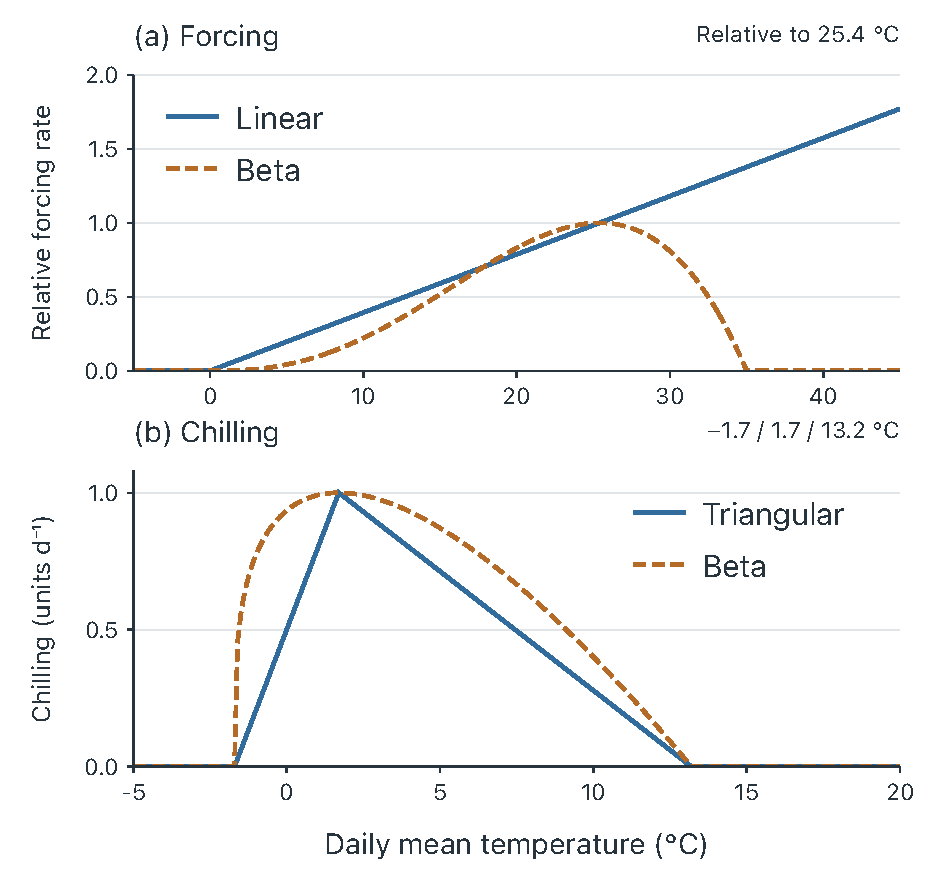
\includegraphics[width=\textwidth,height=0.76\textheight,keepaspectratio]{fig/model_functions/temperature_responses.pdf}
\caption{Fixed temperature-response functions: (a) linear forcing with a 0~$^{\circ}$C base \citep{parkerGeneralPhenologicalModel2011a} and beta forcing with cardinals of 0, 25.4 and 35~$^{\circ}$C; (b) triangular and beta chilling with identical cardinals of $-1.7$, 1.7 and 13.2~$^{\circ}$C. Forcing curves are displayed as $R(T)/R(25.4\,^{\circ}\mathrm{C})$, so both equal one at 25.4~$^{\circ}$C; linear forcing remains uncapped. This display-only normalization does not change model equations or threshold units. Chilling retains native daily response units. Beta parameters follow Fbeta5* and CF10* in \citet{filaComparisonDifferentModelling2014}; transfer to the triangular function of \citet{deWergifosseHETEROFOR2020} is an adaptation. Temperature-axis ranges differ between panels. Accumulation thresholds are calibrated separately and are not shown.}
\label{fig:temperature_responses}
\end{figure}

\paragraph{Joint calibration and numerical safeguards.}
For parameter vector $\symbf{\theta}$ and stage $s$, let $M_s$ denote the number of calibration sites with observations, $n_{js}$ the number of accepted observations at site $j$, and $e_{jsi}(\symbf{\theta})$ the predicted minus observed date for observation $i$, in days. Calibration minimizes

\begin{equation}
L(\symbf{\theta})=\frac{1}{4}\sum_{s\in\mathcal{S}}
\left[\frac{1}{M_s}\sum_{j=1}^{M_s}
\frac{1}{n_{js}}\sum_{i=1}^{n_{js}}
\widetilde{e}_{jsi}(\symbf{\theta})^2\right]^{1/2},
\label{eq:calibration_loss}
\end{equation}

where $\widetilde{e}_{jsi}=e_{jsi}$ for an attained stage and $\widetilde{e}_{jsi}=1000$~d otherwise. Squared errors are averaged within each site and stage, then equally across sites before taking the square root. The four stage-specific RMSEs receive equal weight, regardless of their observation counts. A site or year can contribute any one stage, but all four stages must be represented collectively in the calibration set. Equal weighting does not impose equal errors across stages, and joint fitting can involve trade-offs between budburst and subsequent development.

The implemented optimizer is differential evolution, with three independent restarts using seeds 20260907, 20260908 and 20260909. Each restart uses a population multiplier of 15, a maximum of 300 generations, relative convergence tolerance 0.001, one evaluation worker and no local polishing. Only the four or five continuous accumulation thresholds vary; the fixed response parameters are excluded from optimization through equality bounds or fixed settings. The feasible parameter set with the lowest calibration loss across restarts is retained, without reference to test errors. Restart losses, convergence status, evaluation counts and parameter-boundary proximity are recorded. A saved best candidate is not necessarily a converged solution; convergence and stability under additional calibration-only optimization are prerequisites for interpreting differences as model-structure effects.

Daily weather must be complete and finite throughout the required simulation window. Forcing-only models require coverage from 1 January; chilling models require the preceding 1 September. A common comparison cohort requires coverage sufficient for all ten structures. Missing temperatures are not interpolated. If a stage's forcing requirement is not reached by 31 December, that stage and all subsequent stages remain unpredicted. Unmet chilling also prevents budburst in sequential models, but is not a separate failure condition in parallel models. Fits with no finite prediction for any one observed calibration stage are rejected. The 1000-day penalty enters only the fitting loss, never a synthetic event date or the reported prediction-error metrics. Calendar-date arithmetic preserves leap years and signed dates relative to the target year; previous-year predictions remain visible and are not clipped to January or to the observation-screening windows.

All ten structures enter the paired comparisons in Table~\ref{tab:model_catalogue} without preliminary selection of a single best process model. Their names identify process components and interactions, rather than the parameter-sharing variants compared by \citet{filaComparisonDifferentModelling2014}. Substitution of BBCH07 for that study's BBCH09 target, extension to BBCH89, triangular chilling and the parallel formulations are adaptations requiring independent evaluation. The process-only implementation is available; full-cohort comparisons, residual learning and terrain-effect evaluation remain prospective.

\subsubsection{Residual machine learning}

For observation $i$, the process residual and hybrid prediction are

\begin{equation}
r_i=DOY_{\mathrm{obs},i}-\widehat{DOY}_{\mathrm{proc},i},\qquad
\widehat{DOY}_{\mathrm{hyb},i}=\widehat{DOY}_{\mathrm{proc},i}+\widehat{r}_i.
\label{eq:residual_hybrid}
\end{equation}

Residual models are trained on errors from out-of-fold process predictions within the calibration set. Preprocessing, missing-value treatment, feature selection and hyperparameter tuning are performed within the corresponding training folds. Additional cross-fitting within each inner training set prevents the inner validation observations from influencing residual training. After model selection, the residual learner is fitted using out-of-fold errors from the full calibration set, and the process model is refitted to all calibration observations. Both models are then applied to the independent test set without further fitting.

Predictors are restricted to information available at the time of prediction. Weather summaries for developmental periods use process-predicted stage dates, not observed dates from the validation or test set. Residual correction is applied only when the process model predicts a stage. Variable importance describes predictive associations and does not identify causal physiological mechanisms.

\clearpage
\begingroup
\setstretch{1.0}
\fontsize{11}{13.2}\selectfont
\setlength{\tabcolsep}{3pt}
\setlength{\LTleft}{0pt}
\setlength{\LTright}{\fill}
\renewcommand{\arraystretch}{1.05}
\begin{longtable}{@{}>{\raggedright\arraybackslash}p{0.13\textwidth}>{\raggedright\arraybackslash}p{0.25\textwidth}>{\raggedright\arraybackslash}p{0.18\textwidth}>{\centering\arraybackslash}p{0.07\textwidth}>{\raggedright\arraybackslash}p{\dimexpr0.37\textwidth-8\tabcolsep\relax}@{}}
\caption{Catalogue of the 20 grapevine phenology models evaluated for each stage. F, forcing; C, chilling; ML, residual machine learning. For C + F models, Function gives the forcing / chilling response, in that order. Triangular chilling is the bounded piecewise-linear response in Eq.~\ref{eq:triangular_chilling}. Model codes use L for linear (triangular for chilling), B for beta, S for sequential and P for parallel. The -ML suffix denotes residual correction.}
\label{tab:model_catalogue}\\
\toprule
Process & Function & Interaction & ML & Model name \\
\midrule
\endfirsthead
\caption[]{Complete model catalogue (continued).}\\
\toprule
Process & Function & Interaction & ML & Model name \\
\midrule
\endhead
\midrule
\multicolumn{5}{r}{\footnotesize Continued on next page}\\
\endfoot
\bottomrule
\endlastfoot
Forcing & Linear & --- & No & FL \\
Forcing & Linear & --- & Yes & FL-ML \\
\addlinespace[2pt]
Forcing & Beta & --- & No & FB \\
Forcing & Beta & --- & Yes & FB-ML \\
\addlinespace[2pt]
C + F & Linear / triangular & Sequential & No & CL-FL-S \\
C + F & Linear / triangular & Sequential & Yes & CL-FL-S-ML \\
\addlinespace[2pt]
C + F & Linear / triangular & Parallel & No & CL-FL-P \\
C + F & Linear / triangular & Parallel & Yes & CL-FL-P-ML \\
\addlinespace[2pt]
C + F & Linear / beta & Sequential & No & CB-FL-S \\
C + F & Linear / beta & Sequential & Yes & CB-FL-S-ML \\
\addlinespace[2pt]
C + F & Linear / beta & Parallel & No & CB-FL-P \\
C + F & Linear / beta & Parallel & Yes & CB-FL-P-ML \\
\addlinespace[2pt]
C + F & Beta / triangular & Sequential & No & CL-FB-S \\
C + F & Beta / triangular & Sequential & Yes & CL-FB-S-ML \\
\addlinespace[2pt]
C + F & Beta / triangular & Parallel & No & CL-FB-P \\
C + F & Beta / triangular & Parallel & Yes & CL-FB-P-ML \\
\addlinespace[2pt]
C + F & Beta / beta & Sequential & No & CB-FB-S \\
C + F & Beta / beta & Sequential & Yes & CB-FB-S-ML \\
\addlinespace[2pt]
C + F & Beta / beta & Parallel & No & CB-FB-P \\
C + F & Beta / beta & Parallel & Yes & CB-FB-P-ML \\
\end{longtable}
\endgroup

\subsection{Model evaluation}

\subsubsection{Calibration and test partitioning}

Approximately 80\% of site groups are assigned to calibration and 20\% to testing. Sites are stratified by temperature zones obtained by clustering their climatic profiles across the study area. Monthly ERA5-Land temperatures over a common reference period, provisionally 1991--2020, provide the clustering variables. Zones are defined from raw temperatures and shared by all model comparisons. Climatic clustering uses temperature information only, without phenology observations or prediction errors. Feature scaling, the clustering method, the number of zones and random seeds will be specified before model errors are examined.

Temperature zones are defined independently of country boundaries and are not replaced by temperature-quantile classes. Zones with too few sites are combined according to climatic similarity, or the number of clusters is reduced before evaluation. All years and stages from a site, together with sites sharing an ERA5-Land cell, remain in the same partition. Identical assignments are used across model structures, residual-learning variants and temperature inputs. Four grouped folds within the calibration set support parameter estimation and model selection.

The temperature-zone split assesses prediction at unobserved sites within the sampled climatic range. Additional tests with larger spatial blocks assess regional transfer, while warm-year and warm-site holdouts assess transfer to warmer conditions. Warm years are identified from temperature anomalies using a threshold defined independently of phenology observations. Held-out years and sites are excluded from calibration, residual training and model selection.

\subsubsection{Terrain effects}

Terrain effects on predictive accuracy are assessed using paired predictions at the same held-out sites, years and stages. For each process structure and residual-learning option, the difference in mean absolute error (MAE) between original and DEM-corrected temperature quantifies the contribution of elevation correction; positive values of $MAE_{\mathrm{RAW}}-MAE_{\mathrm{DEM}}$ indicate improved accuracy. Each temperature treatment is calibrated independently on the same calibration observations, so the contrast evaluates correction within the fitted prediction workflow rather than changing temperature while holding process parameters fixed. The correction benefit is compared between process-only and residual-learning models to assess whether the two approaches are complementary.

Paired errors are examined against signed and absolute site-to-grid elevation differences, site elevation, slope, aspect and local elevation variability. Aspect is represented by northness and eastness; terrain summaries and any class boundaries are specified before test errors are examined. Stage-specific contrasts are summarized with equal weight per site, alongside site counts and temperature-zone composition, with uncertainty estimated by paired resampling of independent site groups. Comparisons within temperature zones help distinguish terrain-associated differences from broad climatic contrasts. These analyses describe variation in predictive performance, not causal terrain effects. Improved phenology predictions alone do not establish that corrected temperatures are more accurate; that conclusion requires independent temperature observations.

\subsubsection{Predictive performance and uncertainty}

All parameters are estimated from the calibration set and remain fixed during testing. Temperature input is a separate experimental factor: each of the 20 models in Table~\ref{tab:model_catalogue} is evaluated with original and DEM-corrected temperature, yielding 40 configurations per stage. Paired comparisons use four treatments: process models with raw temperature, hybrid models with raw temperature, process models with corrected temperature and hybrid models with corrected temperature. These comparisons estimate the individual and combined contributions of temperature correction and residual learning, including their interaction. Test observations are used only for performance assessment and subsequent model rankings.

The primary contrasts concern model structure: linear versus beta forcing, absence versus presence of chilling, triangular versus beta chilling, and sequential versus parallel interaction. Corresponding response parameters remain fixed, while accumulation thresholds are recalibrated on identical observations. Function and interaction comparisons within a process family retain the same number of fitted thresholds; including chilling adds one requirement. Calibration and test errors are reported separately for each stage, together with convergence diagnostics. These comparisons quantify predictive differences conditional on the fixed parameterization, rather than assuming that additional processes or parameters guarantee lower error. Lower held-out error supports a benefit from a structural alternative under the specified controls.

With error $e_i=\widehat{DOY}_i-DOY_i$, stage-specific performance is summarized as

\begin{equation}
MAE=\frac{1}{n}\sum_{i=1}^{n}|e_i|,\qquad
RMSE=\sqrt{\frac{1}{n}\sum_{i=1}^{n}e_i^2},\qquad
ME=\frac{1}{n}\sum_{i=1}^{n}e_i.
\label{eq:performance_metrics}
\end{equation}

Positive error indicates a prediction later than the observed date. Performance will be summarized both across observations and with equal weight assigned to each site, together with sample sizes. Uncertainty in paired model differences will be estimated by resampling independent site groups. Where sample sizes permit, errors will also be compared among temperature zones and countries. The frequency of stages not attained because of unmet chilling or forcing requirements is reported separately from errors for finite predicted dates. Sensitivity analyses will examine the effects of phenological screening and an unstratified site split.

\bibliographystyle{plainnat}
\bibliography{references/Phenological}

\end{document}
